\documentclass[12pt]{llncs}

\usepackage[utf8]{inputenc}
\usepackage[T1]{fontenc}
\usepackage{amsmath}
\usepackage{amssymb}
\usepackage{mathtools}
\usepackage{parskip}
\usepackage{tikz}
\usepackage{subcaption}

\usetikzlibrary{arrows}

\captionsetup{compatibility=false}

\DeclarePairedDelimiter\set\{\}

\let\oldleq\leq
\let\covered\prec
\let\incomp\parallel
\let\lext\sqsubseteq
\renewcommand{\implies}{\rightarrow}
\renewcommand{\leq}[1][]{\oldleq_{#1}}
\newcommand{\bicond}{\leftrightarrow}
\newcommand{\poset}[1]{\mathcal{#1}}
\newcommand{\uni}[1][]{\Omega_{#1}}
\newcommand{\lang}[1]{\mathcal{L}(#1)}
\newcommand{\lin}[1]{\texttt{#1}}
\newcommand{\swap}[1][]{\leftrightarrow_{#1}}
\newcommand{\sgraph}[1]{\mathcal{G}(#1)}

\begin{document}

\title{Poset Paper}
\author{Bow-yaw Wang\inst{1} \and Chih-chen Yuan\inst{2}}
\institute{Academia Sinica, Taiwan\\ \and
National Taiwan Normal University, Taiwan\\}
\maketitle

\begin{abstract}
hello world
\end{abstract}

\section{Introduction}
Intro part here

\section{Preliminaries}
A \emph{partial order} is a binary relation that is reflexive, antisymmetric, and transitive. A partially ordered set or poset is a binary structure $\poset{P} = (\uni, \leq)$ where the \emph{universe} $\uni$ is a set and $\leq$ is a partial order on $\uni$; we refer to members of $\uni$ as elements of $\poset{P}$ and, where specificity is desired, to $\uni$ as $\uni[
\poset{P}]$ and $\leq$ as $\leq[\poset{P}]$.

% example:posetp
\begin{example}
    For the following definition, consider the poset $\poset{P}$ over $\set{a,b,c,d}$ with $a \leq b$; $a \leq c$; $a \leq d$; $b \leq d$; and $c \leq d$. Figure~\ref{figure:posetp} describes $\poset{P}$ with a graph $(V,E) = (\Omega,\covered)$.
    \label{example:posetp}
\end{example}

% figure:posetp
\begin{figure}
    \centering
    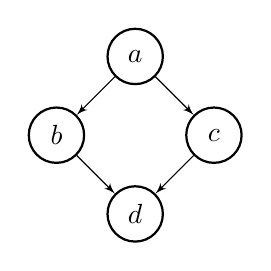
\begin{tikzpicture}
        [
        vertex/.style={circle,thick,draw,minimum size=2em},
        edge/.style={->,> = latex'}
        ]
    \node[vertex] (1) at (1,2) {$a$};
    \node[vertex] (2) at (0,1) {$b$};
    \node[vertex] (3) at (2,1) {$c$};
    \node[vertex] (4) at (1,0) {$d$};
    \draw[edge] (1) -- (2);
    \draw[edge] (1) -- (3);
    \draw[edge] (2) -- (4);
    \draw[edge] (3) -- (4);
    \end{tikzpicture}
    \caption{Graph representation of $\poset{P}$ from Example~\ref{example:posetp}.}
    \label{figure:posetp}
\end{figure}

The \emph{cover} relation $\covered$ of a poset $\poset{P}$ is the transitive reduction of the order relation; it describes the case of immediate successor: for $x, y \in \poset{P}$, $x \covered y$ iff $x \leq y \wedge \not\exists z \in \poset{P}, x \leq z \wedge z \leq y$. For Example~\ref{example:posetp}, the covered relation includes $a \covered b$; $a \covered c$; $b \covered d$; and $c \covered d$. Note that $(a,d)$ is absent in $\covered$.

In addition, we describe the case of \emph{incomparability} in a poset $\poset{P}$ with $\incomp$: for $x, y \in \poset{P}$, $x \incomp y$ iff $x \not\leq y \wedge y \not\leq x$. For Example~\ref{example:posetp}, there is $b \incomp c$.

% example:posetl
\begin{example}
    For the following definition, consider the poset $\poset{L}$ over $\set{a,b,c,d}$ with $a \leq b$; $a \leq c$; $a \leq d$; $b \leq c$; $b \leq d$; and $c \leq d$. Figure~\ref{figure:posetl} represents $\poset{L}$ with a graph $(V,E) = (\uni,\covered)$.
    \label{example:posetl}
\end{example}

% figure:posetl
\begin{figure}
    \centering
    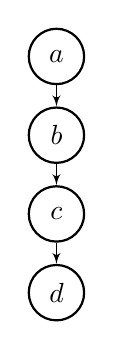
\begin{tikzpicture}
        [
        vertex/.style={circle,thick,draw,minimum size=2em},
        edge/.style={->,> = latex'}
        ]
    \node[vertex] (1) at (0,3) {$a$};
    \node[vertex] (2) at (0,2) {$b$};
    \node[vertex] (3) at (0,1) {$c$};
    \node[vertex] (4) at (0,0) {$d$};
    \draw[edge] (1) -- (2);
    \draw[edge] (2) -- (3);
    \draw[edge] (3) -- (4);
    \end{tikzpicture}
    \caption{Graph representation of $\poset{L}$ from Example~\ref{example:posetl}.}
    \label{figure:posetl}
\end{figure}

A partial order that is also total is called a \emph{linear order}; every pair of elements are comparable in a linear order. Note that the graph describing a linear order is a path graph. For simplicity, we represent a linear order in string form. For Example~\ref{example:posetl}, we write \lin{abcd}.

For a poset $\poset{P}$, a linear order $\poset{L}$ that extends $\poset{P}$ is called a \emph{linear extension} or \emph{linearization} of $\poset{P}$, and we write $\poset{P} \lext \poset{L}$ iff $\poset{L}$ is a linearization of $\poset{P}$. For example, for $\poset{P}$ from Example~\ref{example:posetp} and $\poset{L}$ from Example~\ref{example:posetl}, $\poset{P} \lext \poset{L}$. Note that a linearization of a poset is equivalent to a topological sort of the graph describing that poset.

The set of all linearizations of $\poset{P}$ is denoted $\lang{\poset{P}}$. We shall consider it the \emph{language} of a poset. For $\poset{P}$ from Example~\ref{example:posetp}, $\lang{\poset{P}} = \set{\lin{abcd},\lin{acbd}}$.

Now, we are ready to give the problem definition of the \emph{Poset Cover Problem}.

% definition:pcp
\begin{definition}[Poset Cover Problem]
    Given a set of linear orders $\Upsilon$, find a set of partial orders $C$, called a cover, such that $|C|$ is minimal and $\Upsilon = \bigcup_{\poset{P} \in C} \lang{\poset{P}}$.
    \label{definition:pcp}
\end{definition}

% example:cover example
\begin{example}
    Given the set of linear orders $\set{\lin{abfce},\lin{bafce},\lin{abcfe},\lin{abfec}}$ over $\set{a,b,c,f,e}$, a minimal poset cover $C$ of two posets $\poset{A},\poset{B}$ is shown in Figure~\ref{figure:cover example c} with ${\lang{\poset{A}} = \set{\lin{abfce},\lin{abcfe},\lin{abfec}}}$ and ${\lang{\poset{B}} = \set{\lin{bafce}}}$.
    \label{example:cover example}
\end{example}

% figure:cover example
\begin{figure}
    % figure:cover example c
    \begin{subfigure}[b]{0.5\textwidth}
        \centering
        \begin{subfigure}[b]{0.4\textwidth}
            \centering
            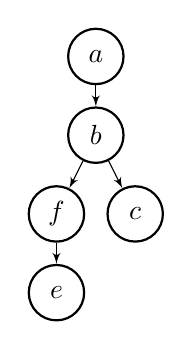
\begin{tikzpicture}
                [
                vertex/.style={circle,thick,draw,minimum size=2em},
                edge/.style={->,> = latex'}
                ]
            \node[vertex] (1) at (1,4) {$a$};
            \node[vertex] (2) at (1,3) {$b$};
            \node[vertex] (3) at (0.5,2) {$f$};
            \node[vertex] (4) at (0.5,1) {$e$};
            \node[vertex] (5) at (1.5,2) {$c$};
            \draw[edge] (1) -- (2);
            \draw[edge] (2) -- (3);
            \draw[edge] (3) -- (4);
            \draw[edge] (2) -- (5);
            \end{tikzpicture}
            \caption{Poset $\poset{A}$.}
        \end{subfigure}%
        \begin{subfigure}[b]{0.4\textwidth}
            \centering
            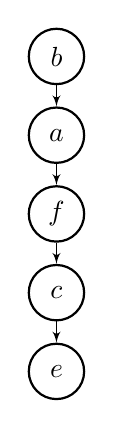
\begin{tikzpicture}
                [
                vertex/.style={circle,thick,draw,minimum size=2em},
                edge/.style={->,> = latex'}
                ]
            \node[vertex] (6) at (4,4) {$b$};
            \node[vertex] (7) at (4,3) {$a$};
            \node[vertex] (8) at (4,2) {$f$};
            \node[vertex] (9) at (4,1) {$c$};
            \node[vertex] (10) at (4,0) {$e$};
            \draw[edge] (6) -- (7);
            \draw[edge] (7) -- (8);
            \draw[edge] (8) -- (9);
            \draw[edge] (9) -- (10);
            \end{tikzpicture}
            \caption{Poset $\poset{B}$.}
        \end{subfigure}
        \caption{Cover $C$.}
        \label{figure:cover example c}
    \end{subfigure}%
    % figure:cover example c'
    \begin{subfigure}[b]{0.5\textwidth}
        \centering
        \begin{subfigure}[b]{0.4\textwidth}
            \centering
            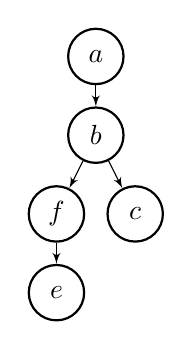
\begin{tikzpicture}
                [
                vertex/.style={circle,thick,draw,minimum size=2em},
                edge/.style={->,> = latex'}
                ]
            \node[vertex] (1) at (1,4) {$a$};
            \node[vertex] (2) at (1,3) {$b$};
            \node[vertex] (3) at (0.5,2) {$f$};
            \node[vertex] (4) at (0.5,1) {$e$};
            \node[vertex] (5) at (1.5,2) {$c$};
            \draw[edge] (1) -- (2);
            \draw[edge] (2) -- (3);
            \draw[edge] (3) -- (4);
            \draw[edge] (2) -- (5);
            \end{tikzpicture}
            \caption{Poset $\poset{C}$.}
        \end{subfigure}%
        \begin{subfigure}[b]{0.4\textwidth}
            \centering
            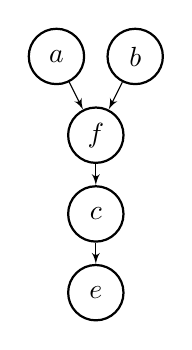
\begin{tikzpicture}
                [
                vertex/.style={circle,thick,draw,minimum size=2em},
                edge/.style={->,> = latex'}
                ]
            \node[vertex] (6) at (3.5,4) {$a$};
            \node[vertex] (7) at (4.5,4) {$b$};
            \node[vertex] (8) at (4,3) {$f$};
            \node[vertex] (9) at (4,2) {$c$};
            \node[vertex] (10) at (4,1) {$e$};
            \draw[edge] (6) -- (8);
            \draw[edge] (7) -- (8);
            \draw[edge] (8) -- (9);
            \draw[edge] (9) -- (10);
            \end{tikzpicture}
            \caption{Poset $\poset{D}$.}
        \end{subfigure}
        \caption{Cover $C'$.}
        \label{figure:cover example c'}
    \end{subfigure}
    \caption{Minimal covers for the set $\set{\lin{abfce},\lin{bafce},\lin{abcfe},\lin{abfec}}$.}
    \label{figure:cover example}
\end{figure}

Note that a minimal poset cover may not be unique and the languages of the posets in a cover may overlap. For Example~\ref{example:cover example}, there is another minimal poset cover $C'$ shown in Figure~\ref{figure:cover example c'} with overlapping languages of posets $\poset{C},\poset{D}$ with ${\lang{\poset{C}} = \set{\lin{abfce},\lin{abcfe},\lin{abfec}}}$ and ${\lang{\poset{D}} = \set{\lin{abfce},\lin{bafce}}}$.

\section{Swap Graph}
% NOTE: redo
Since the poset cover problem is proved to be NP-complete, we decided to utilize the power of SAT solvers. However, a naive encoding would easily result in superpolynomial reduction. An efficient encoding requires some preprocessing using notions introduced as follows.

% put naive here?

The \emph{swap} relation $\swap$ describes the case of ``off by one swap'' between linear orders with shared universe: for linear orders $\poset{L}_1$~and~$\poset{L}_2$, $\poset{L}_1~\swap~\poset{L}_2$ iff there are $x, y \in \uni$ such that $\leq[\poset{L}_1] \cap \leq[\poset{L}_2] = {(\leq[\poset{L}_1] \cup \leq[\poset{L}_2])} - \set{(x,y),(y,x)}$; where specificity is desired, we write $\swap[x,y]$. For example, \lin{abcd} $\swap[b,c]$ \lin{acbd}. Note that $\swap$ is symmetric.

For a set of linear orders $\Upsilon$, the \emph{swap graph} $\sgraph{\Upsilon}$ of it is the undirected graph $(V,E) = (\Upsilon,\swap)$. Figure~\ref{figure:graphlp} shows the swap graph of $\lang{\poset{P}}$ for $\poset{P}$ from Example~\ref{example:posetp}. The swap graph of the linearizations of a single poset is connected.

% figure:graphlp
\begin{figure}
    \centering
    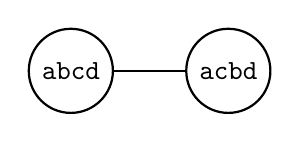
\begin{tikzpicture}
        [
        vertex/.style={circle,thick,draw,minimum size=2em},
        edge/.style={thick}
        ]
    \node[vertex] (1) at (0,0) {\lin{abcd}};
    \node[vertex] (2) at (2,0) {\lin{acbd}};
    \draw[edge] (1) -- (2);
    \end{tikzpicture}
    \caption{Swap graph of $\lang{\poset{P}}$ for $\poset{P}$ from Example~\ref{example:posetp}.}
    \label{figure:graphlp}
\end{figure}

We use the property that swap graphs are connected to avoid the exponential result of naive encoding.

% put proposition here?

% put new encoding here?

% where to put sat iff proof?

%########################################

\section{Problem Definition?or Poset covered Problem}
intro pcp; intro converse of lin; intro trivial non-max solution? intro np completeness?

The poset covered problem is: given a set of linearizations $\Upsilon$, find a set of posets $\mathcal{C}$, called a covered, such that $\Upsilon = \bigcup_{P \in C} \mathcal{L}(P)$ and that $|\mathcal{C}|$ is minimal.

\begin{theorem}
    insulating barrier method where?
\end{theorem}

\section{SAT Encoding Part}
We use the boolean logic of z3 SMT solver from MS research. Since poset is connected, by contraposition, we can first divide and conquer on connected components of the swap graph, by solving each component individually.

We then check with incrementing number of posets to find the minimal number of posets to covered each component. We first encode the axioms of posets; namely, reflexivity, antisymmetry, and transitivity. Next, we encode the extension constraint with contraposition from input linearizations to reduce the number of variables. Finally, we encode the non-extension constraint with negation of extension constraint on the insulating barrier.

\section{Exp Part}
NOTE: how do i put graph here?

\section{Conclusions}

\section{References}
NOTE: how to use list?

\section{Appendix}

\begin{theorem}
    Permutations and Nerode
\end{theorem}

\begin{theorem}
    (Corollary of Szpilrajn extension theorem) For a partial order $\leq$, $\leq = \bigcap_{< \in \mathcal{E}(\leq)} <$.
\end{theorem}

\begin{theorem}
    (Heath and Nema) If $x \incomp y$ for $\leq$ and there is $< \in \mathcal{E}(\leq)$ such that $x \covered y$ for $<$, then there is $<' \in \mathcal{E}(\leq)$ such that $y \covered x$ for $<'$.
\end{theorem}

\begin{theorem}
    Swap graphs are connected by Kendall tau paths
\end{theorem}

\begin{theorem}
    %(Szpilrajn Theorem) For a partial order $\poset{P}$, there exists a linear order $\mathcal{L}$ that extends $\poset{P}$; that is, $\leq_{\poset{P}} \subseteq \leq_{\mathcal{L}}$.
    \label{theorem:szpilrajn}
\end{theorem}

\begin{theorem}
    (Pruesse? and Ruskey) For a poset $\poset{P}$, the swap graph $\mathcal{G}(\poset{P})$ is connected. cite???
\end{theorem}

That's it? should we move the swap things to motivations?

\end{document}
